This chapter presents methods used to evaluate the system and the results collected evaluating the system. 

\section{Methods}
\subsection{User Survey}

The system is measured by doing user surveys on the end users. In our user survey we have coaches’ rating how much they agree with a statement on a Likert-scale. The statements compare the system against other systems in use at Alfheim today. The Likert-scale chosen is a 5 point scale from \textit{strongly disagree} to \textit{strongly agree}.\footnote{http://www.simplypsychology.org/likert-scale.html}. In short it will let each individual to note how much they disagree or agree with a particular statement.

\subsection{UI Performance}

Measuring \ac{UI} Performance is way of measuring usability of the system. These two are directly linked up to each other \cite{satisfaction}. A slow system and unresponsive system decrease satisfaction and usability for the end-user. Founding in \cite{nielsen} indicated that a response time of longer than 1000ms would decrease the satisfaction of the user. The thought-flow of the user will not be interrupted and therefor one can argue it's fast enough. We will use this threshold to evaluate our system. 

To measure the UI Performance we use Google Chrome DevTools\footnote{https://developers.google.com/chrome-developer-tools/}. A web page is only fully loaded when all requests have been received. In our system new requests will be spawned after the \ac{DOM}. We test both a fully reload of the page and when the users navigate.

\section{Experiments and Results}

In the tests \ac{TIL} have been used to evaluate the system. In the tests we are after is to see if we have achieved or goals listed in the requirements. To recapture the main goals; we wanted to identify key players in soccer opponent teams and we wanted to create a system that difference it from the existing systems and at the same time provides valuable information for opponent soccer analytic. 

\subsection{Test data and Assessors}

In the evaluation phase the database had been populated with data from \ac{TIL} and Str{\o}msgodset matches. Only attacks from these two teams have been used in the evaluating process. A total of 34 attacks have been captured for Str{\o}msgodset over 5 matches. For \ac{TIL} a total of 42 attacks have been captured over 9 matches. Figure \ref{fig:matches_regged} lists all matches. Some matches include data from other teams than \ac{TIL} and Str{\o}msgodset. They have not been taken into consideration in the evaluating process.

\begin{figure}[ht!]
\centering
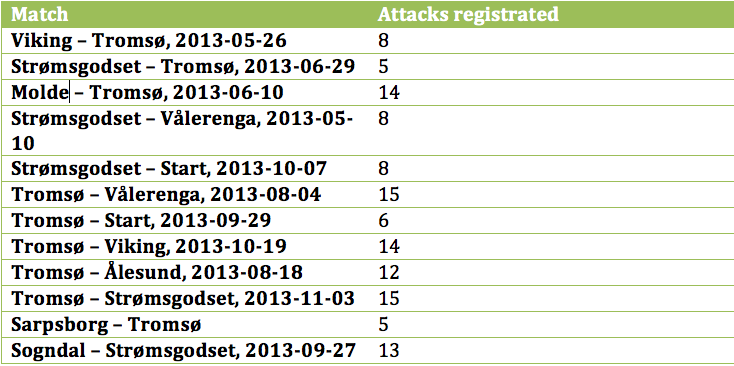
\includegraphics[width=1\textwidth]{images/general/matched_regged.png}
\caption{Matches that have been captured and persisted into the database}
\label{fig:matches_regged}
\end{figure}

\subsection{SAT as a tool for opponent analytic}
% SAT gives you valuable information about opponents that the current systems you use today don’t provide

In this User Servey the assessors where asked how SAT is as a complementary opponent analytic tool. In the requirement process we specified that the system should to be a complementing tool and not a direct replacement of the systems in use. The results shows that most of the assessors values what the system provides. 

Assessors not in the Tromsø IL system do not necessarily use or have experience with an existing tool. Therefor the statement was re-phrased. The assessors were asked how SAT is as an opponent analytic tool, a stand-alone product. The results shows

From these results we can conclude that the end-users view the Soccer Analytic Tool as a good system to complement with for opponent analytic.

\subsection{SAT as a tool for identifying key players}

In this User Servey the assessors where asked how SAT is as a tool for identifying key players in a soccer team. This was one of the main goals of the system. We can see from the results of the User Servey that the system identifies key players well. All votes for ¨strongly agree¨. 

\subsection{UI-performance}
UI performance was measured by testing the most content rich web page the team analytic page for \ac{TIL}. All the response times were measured by doing 20 samples. Tests where run at localhost with server and database running on the same machine, meaning that a further increase in time would likely be seen if the system was in production. 

In \ac{SPA} you don’t necessary get all the files at once, but when you need them. On render, the web browser will first get the root \ac{HTML} document and then start requesting all other files that is referenced. JavaScript files can in theory be bundled to one file saving some network traffic. JavaScript files our system the query with the longest run time is the team statistics query and this is run when you visit a team page. When doing a clean reload of the page (non 303 Not Modified status codes) Google Developer Tools reports that total 55 requests is done to the back-end.

\subsection{Database size}
In figure \ref{fig:dbsize} the size of the different indexes in the database is listed. Match related data is stored in the match, attack and pass index. The total size of those 3 indexes is 379.5kb and with a total of 12 matches. This means that an average match takes around 31.6kb of storage.

\begin{figure}[ht!]
\centering
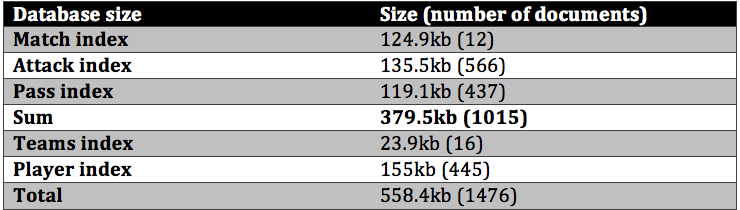
\includegraphics[width=1\textwidth]{images/evaluation/dbsize}
\caption{Table with the size of each index and total size}
\label{fig:dbsize}
\end{figure}


\section{Discussion}
\subsection{Input}

Perhaps the biggest limitation of the system is that it requires manual work to be functional. The system requires a lot of manually work to be operational as an opponent analytic tool. Up to one hour is the normal time spent capturing all data for a match with the current capture interface. On average, teams across the top four top leagues (La Liga, Premier League, Serie A and Bundesliga) took about 13 shots per match, measured in the 2010/11 season \cite{soccerbynumbers}. This means you will have possible have 26 attacks to capture.

In section \ref{sec:capprocess} it is mentioned that you have to store the players by their ID. IDs are only found in the database. Instead of this a player selector interface could have been developed letting you just click on a image of the player involved. We suggest you can save up to 20 minutes by having this feature added.

There is minimal quality checking of the input data except from the match view page that lists every attack captured, meant for external operators to verify the data. Other than that you have to trust the operator that is capturing match data. The input is to some degree subjective for some data like identifying breakthroughs. In some situations one operator may say that it was a breakthrough and another wouldn't agree. This may not be the biggest problem if you set some rules to follow for the operators.

An average match is around 31.6kb size large. In comparison with ZXY a match is around 500-700mb. A better comparison would be against Opta as they are more in the genre of our system with only manual input. As previously mentioned, they capture every pass in the game meaning that they most likely stores more.

\subsection{Domain model}
The domain model has been dedicated a lot of time to in the process. It was crucial to have a domain model that reflected what type of opponent analytic information the system should give the end-user. However, having many things to capture increases time spent in the process of capturing data. 

A thing that should have been changed to get more precise data is how breakthroughs are represented in the database. The current solutions store each type of breakthrough as text saying where on the pitch it came from. Rather than this we could have taken advantage of the dividing of the pitch we already have. This would have given use more precise data.

\subsection{Interfaces}

One comment from an end user was about the graphical components illustrating statistics on the client. Improving the graphical components would increase the overall experience of the system. This has not been one of the main focuses during the development of the system.

\subsection{UI Performance}

\subsection{Scalability}





